% Results
\section{Results}
\label{sec:results}

We summarize quantitative comparisons and highlight representative qualitative cases.
Figures referenced below are produced by our analysis scripts and included under \texttt{paper/figures/}.

\subsection{Ablation Study}
\label{sec:ablation}

Table~\ref{tab:ablation-summary} summarizes key ablations.
As expected, removing the table agent (\texttt{no\_table}) eliminates tables (\(S_{\mathrm{tab}}\) drops from 1.0 to 0.0; corrected \(q<0.01\)), validating that our ablation controls are functioning and that the table component causally affects tabular structure.
Other ablations show comparatively small changes on most metrics, suggesting the full system's structural completeness is robust for this benchmark.

% Auto-generated table (small subset)
% Auto-generated by scripts/export_paper_assets.py
\begin{table*}[t]
\centering
\small
\setlength{\tabcolsep}{4pt}
\begin{tabular}{lrrrrrr}
\toprule
Metric & Full & no\_table & no\_consistency & no\_alignment & no\_vision & async\_queue \\
\midrule
S\_sem & 0.8805 & 0.8805 & 0.8778 & 0.8805 & 0.8750 & 0.8805 \\
S\_ps & 1.0000 & 1.0000 & 1.0000 & 1.0000 & 1.0000 & 1.0000 \\
S\_uj & 1.0000 & 0.9778 & 0.9778 & 0.9704 & 0.9778 & 1.0000 \\
S\_hyp & 1.0000 & 1.0000 & 1.0000 & 1.0000 & 1.0000 & 1.0000 \\
S\_tab & 1.0000 & \textbf{0.0000} & 1.0000 & 0.9333 & 0.9333 & 1.0000 \\
S\_bi & 0.5074 & 0.5631 & 0.5639 & 0.5636 & 0.5615 & 0.5583 \\
\bottomrule
\end{tabular}
\caption{Ablation summary (means over 15 briefs). Removing the Table agent (\texttt{no\_table}) eliminates tables by design (bold).}
\label{tab:ablation-summary}
\end{table*}


\subsection{Full System vs. StrongPrompt Baseline}
\label{sec:baseline}

Table~\ref{tab:full-vs-strong} compares the full system with \textsc{StrongPrompt}.
The full system achieves statistically significant gains (Holm--Bonferroni corrected) on deliverability-oriented metrics:
\(S_{\mathrm{ps}}\) (\(\Delta=+0.6811\), \(q=0.0060\)),
\(S_{\mathrm{uj}}\) (\(\Delta=+0.6389\), \(q=0.0066\)),
and \(S_{\mathrm{hyp}}\) (\(\Delta=+0.6000\), \(q=0.0066\)).
For semantic quality \(S_{\mathrm{sem}}\), the full system improves the mean (\(\Delta=+0.1083\)) but is not significant after correction (\(q=0.0639\)).
We observe a trade-off on bilingual compliance \(S_{\mathrm{bi}}\): \textsc{StrongPrompt} scores higher (\(\Delta=-0.0672\), \(q=0.0013\)), indicating that stricter bilingual prompting can improve bilingual formatting consistency.

% Auto-generated by scripts/export_paper_assets.py
\begin{table}[t]
\centering
\small
\setlength{\tabcolsep}{4pt}
\begin{tabular}{lrrrr}
\toprule
Metric & Full & StrongPrompt & $\Delta$ & $q$ \\
\midrule
S\_sem & 0.8805 & 0.7722 & 0.1083 & 0.0639 \\
S\_ps & 1.0000 & 0.3189 & 0.6811 & \textbf{0.0060} \\
S\_uj & 1.0000 & 0.3611 & 0.6389 & \textbf{0.0066} \\
S\_hyp & 1.0000 & 0.4000 & 0.6000 & \textbf{0.0066} \\
S\_bi & 0.5597 & 0.6269 & -0.0672 & \textbf{0.0013} \\
S\_tab & 1.0000 & 1.0000 & 0.0000 & 1.0000 \\
S\_biz & 0.5000 & 0.5111 & -0.0111 & 1.0000 \\
S\_tech & 1.0000 & 1.0000 & 0.0000 & 1.0000 \\
S\_risk & 1.0000 & 1.0000 & 0.0000 & 1.0000 \\
S\_comp & 1.0000 & 1.0000 & 0.0000 & 1.0000 \\
S\_mm & 1.0000 & 1.0000 & 0.0000 & 1.0000 \\
S\_expert & 1.0000 & 1.0000 & 0.0000 & 1.0000 \\
S\_var & 0.0000 & 0.0000 & 0.0000 & 1.0000 \\
\bottomrule
\end{tabular}
\caption{Full system vs. StrongPrompt baseline on 15 briefs. $\Delta$ = Full $-$ StrongPrompt. $q$ is Holm--Bonferroni corrected Wilcoxon p-value.}
\label{tab:full-vs-strong}
\end{table}


\subsection{Qualitative Case Study (Three-way)}
\label{sec:case}

We include a three-way case study (full system vs. \texttt{no\_table} vs. \textsc{StrongPrompt}) on representative briefs.
Across cases, the full system tends to produce clearer separation between problem statements and solution design, and more complete user-journey artifacts, while \textsc{StrongPrompt} often yields shorter sections and weaker journey grounding despite matching structural checklists.
Removing tables predictably harms tabular summaries while keeping most narrative sections intact.

\paragraph{Figures.}
We provide plots for aggregate comparisons:
Figure~\ref{fig:full-strong} (Full vs. StrongPrompt) and Figure~\ref{fig:ablation-heatmap} (ablation heatmap).

\begin{figure}[t]
  \centering
  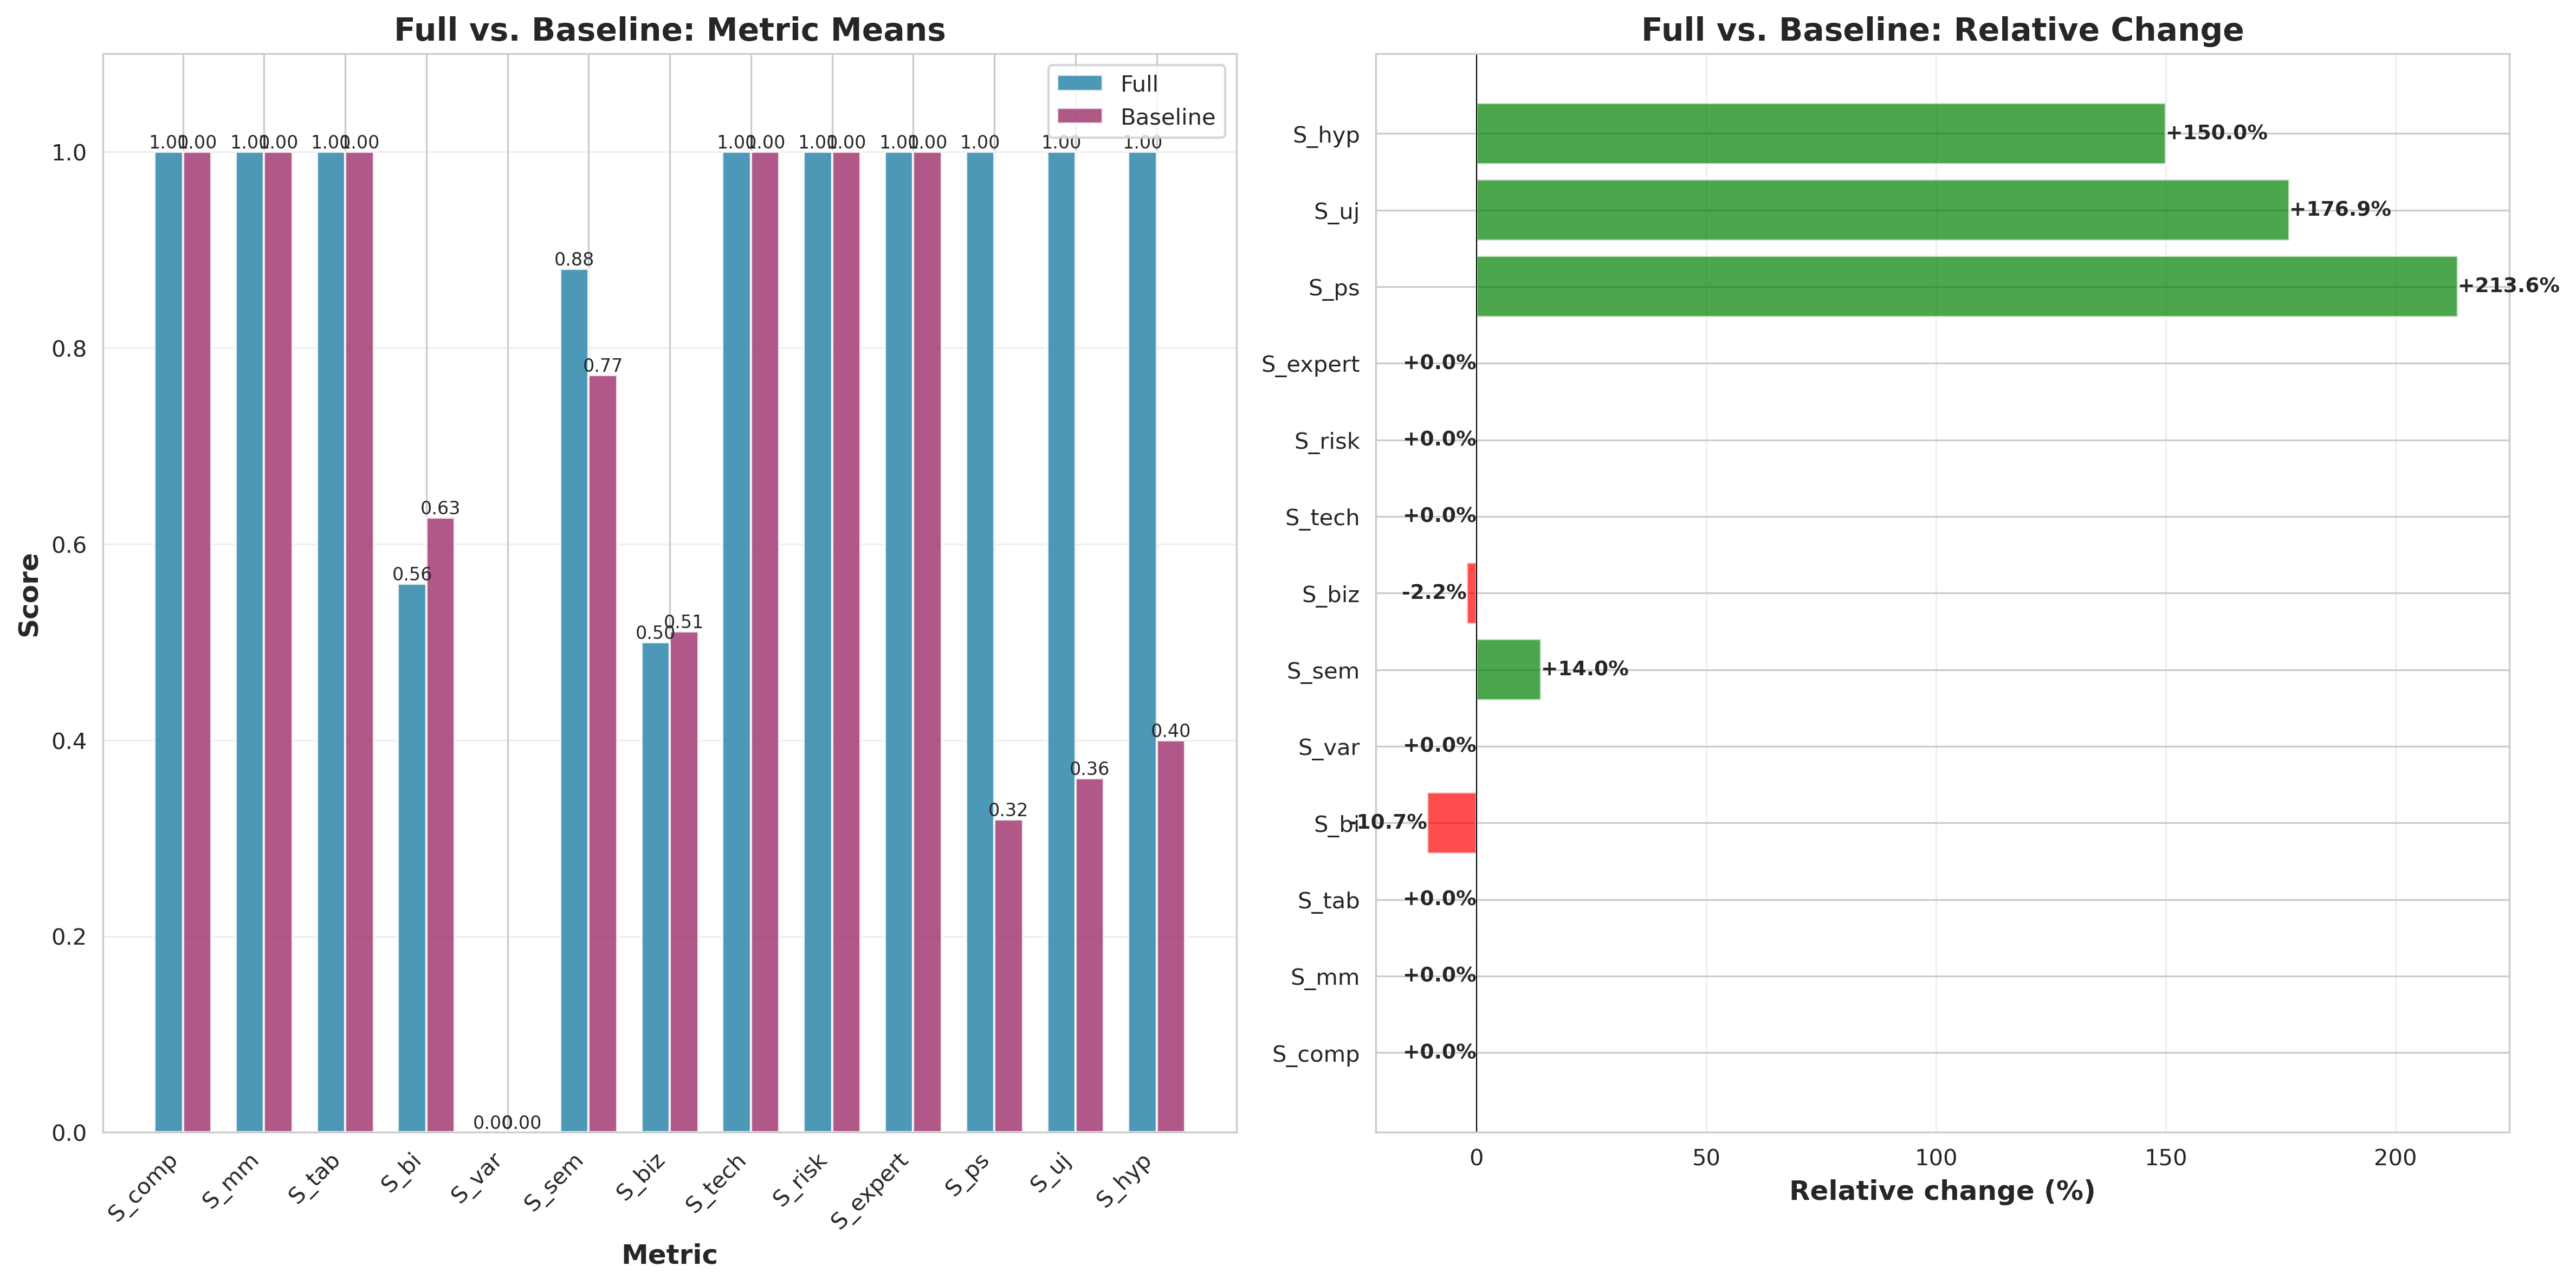
\includegraphics[width=\columnwidth]{figures/full_vs_strong_prompt_comparison.png}
  \caption{Full system vs. StrongPrompt baseline across metrics (means over 15 briefs).}
  \label{fig:full-strong}
\end{figure}

\begin{figure}[t]
  \centering
  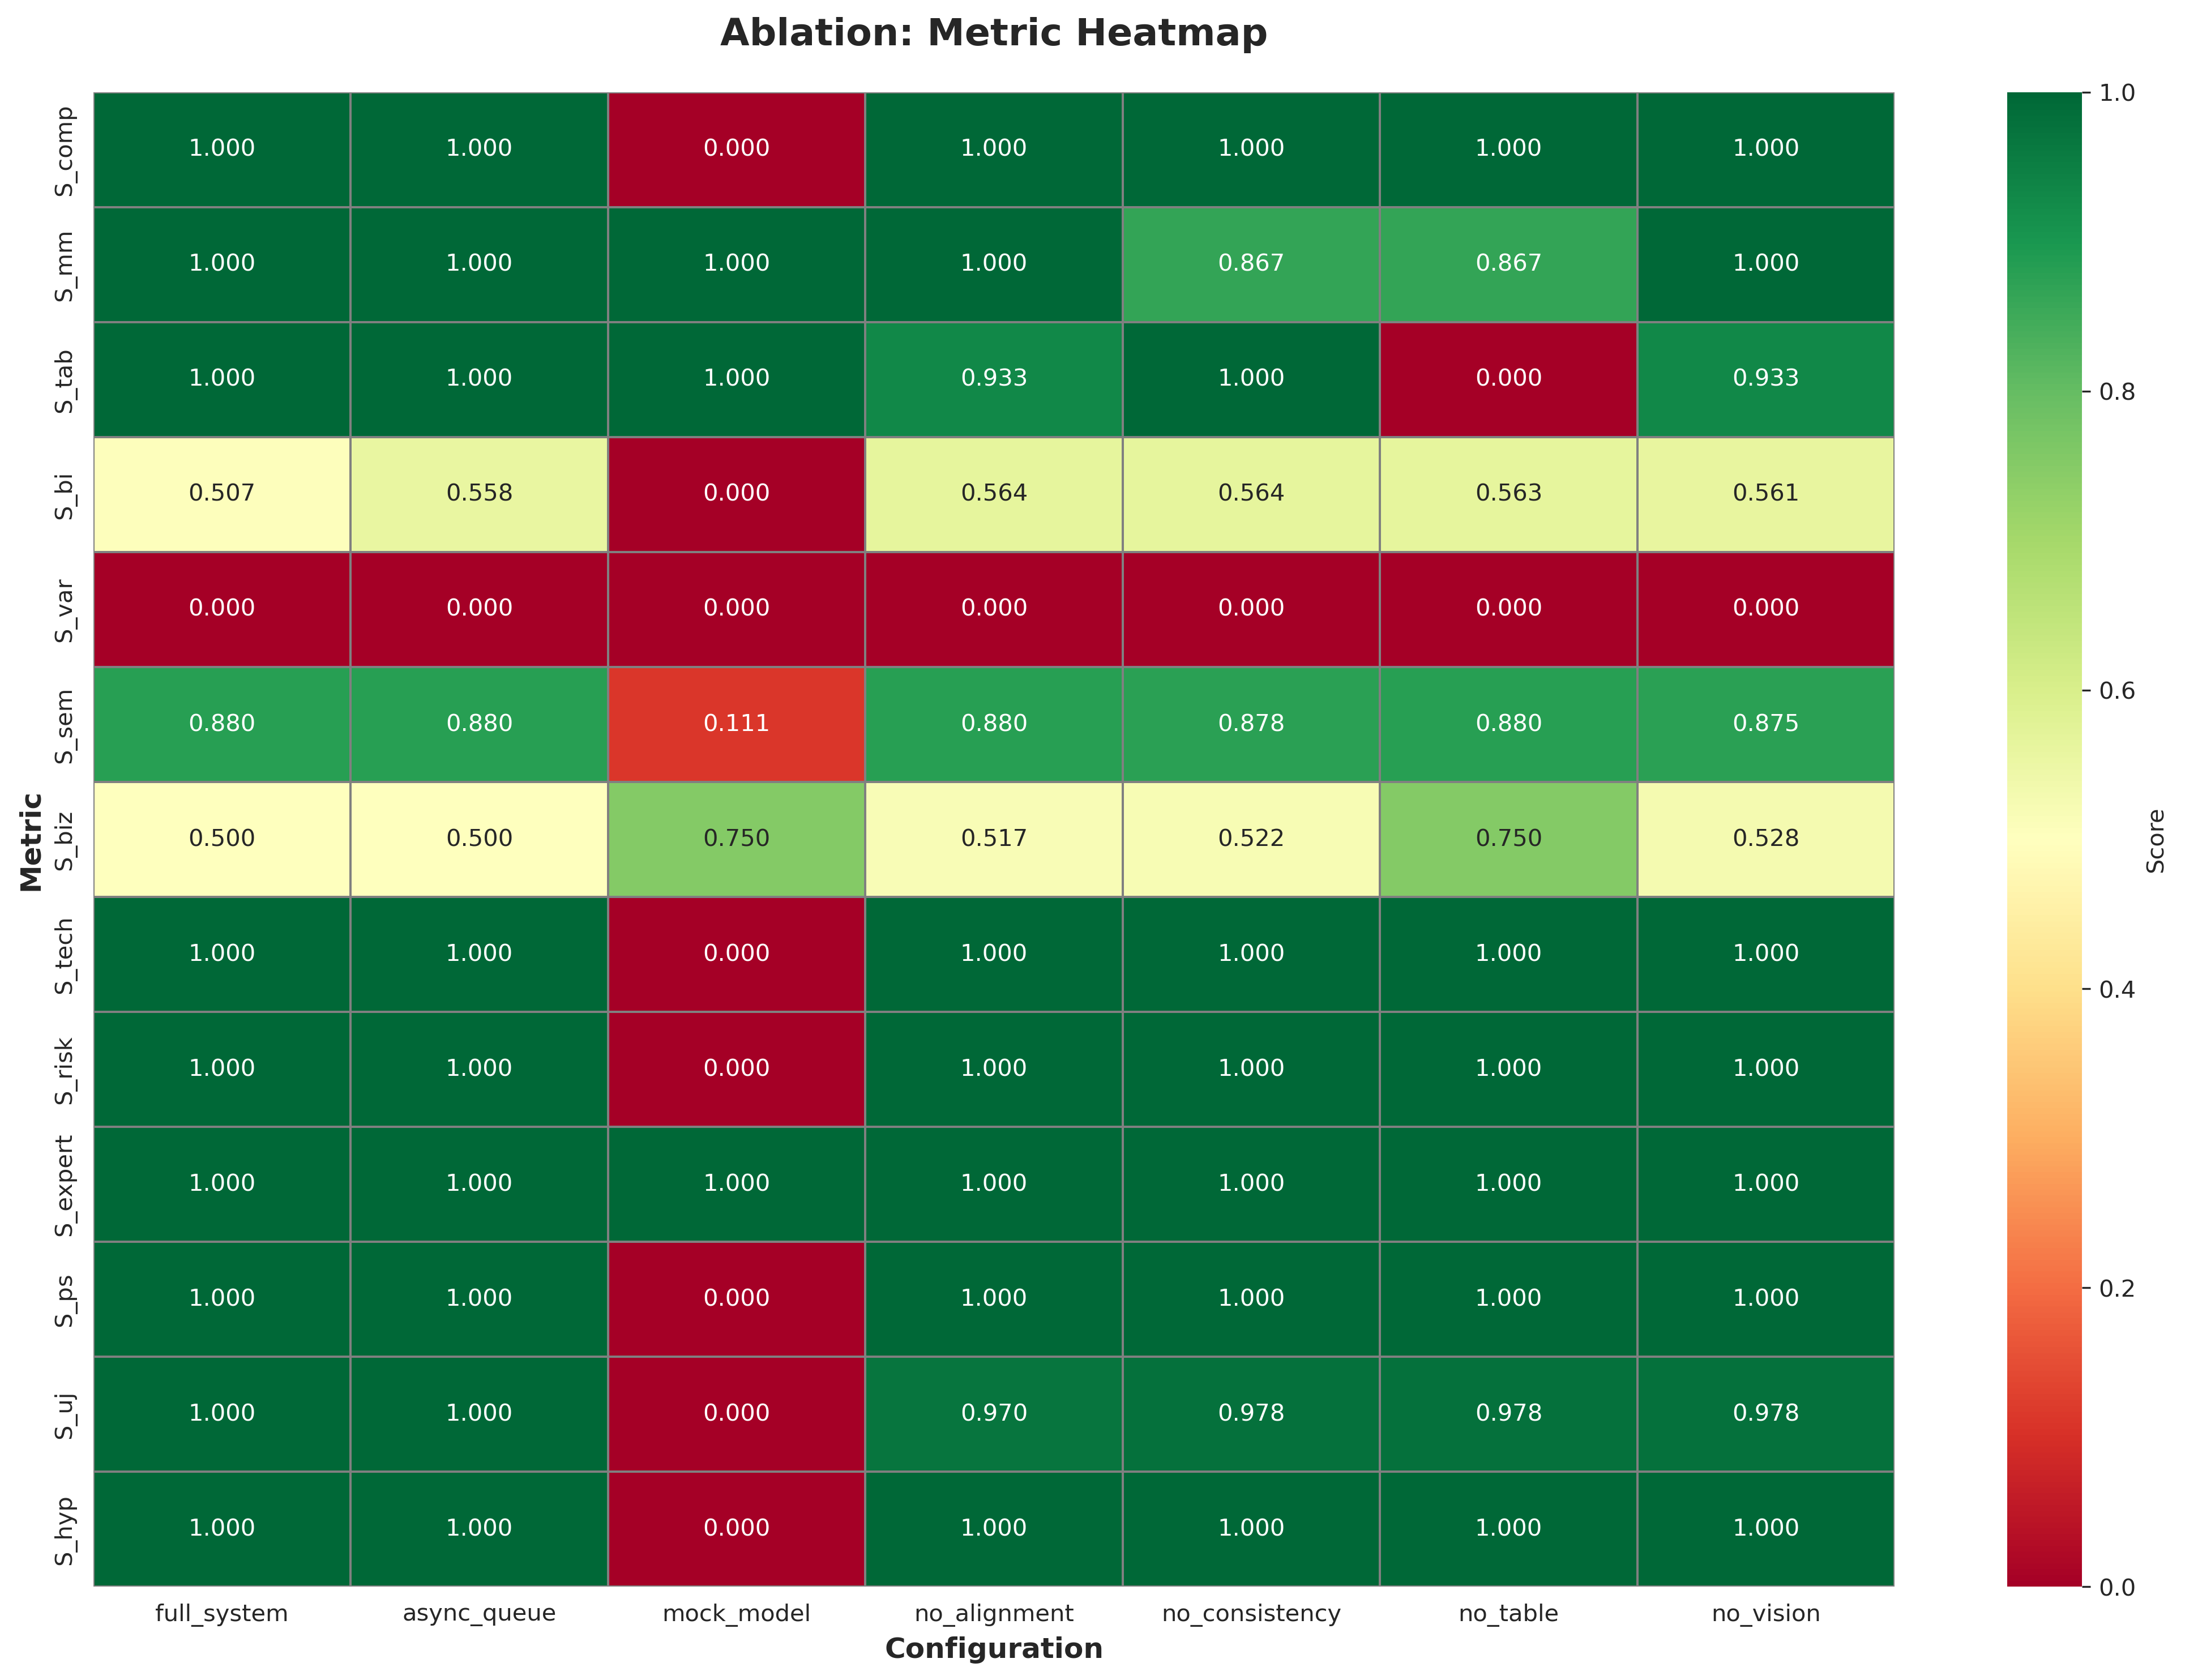
\includegraphics[width=\columnwidth]{figures/ablation_heatmap.png}
  \caption{Ablation heatmap: mean metric values per configuration (15 briefs).}
  \label{fig:ablation-heatmap}
\end{figure}


